\documentclass[12pt,aspectratio=43]{beamer}

%%%%%%%%%%%%%%%%%%%%%%%%%%%%%%%%%%%%%%%%%%%%%%%%%%
%   Paquetes de configuración basica del texto   %
%%%%%%%%%%%%%%%%%%%%%%%%%%%%%%%%%%%%%%%%%%%%%%%%%%
\usepackage[spanish,es-nodecimaldot]{babel}
\usepackage{babelbib}
\usepackage[T1]{fontenc}
\usepackage{listings}
\usepackage{multirow}
\usepackage{hyperref}
\usepackage{hyperxmp}
\usepackage{ifthen}

%%%%%%%%%%%%%%%%%%%%%%%%%%%%%%%%%%%%%%%%%%%%%%%%%%
%                   [listings]                   %
%   Configuración de vizualizacion del código    %
%%%%%%%%%%%%%%%%%%%%%%%%%%%%%%%%%%%%%%%%%%%%%%%%%%
\lstset{
	backgroundcolor=\color{lightgray!10},
	basicstyle=\ttfamily,
	extendedchars=true,
	showspaces=false,
	showstringspaces=false,
	captionpos=b,
	keywordstyle=\bfseries\color{cyan},
	commentstyle=\color{gray},
	stringstyle=\color{orange},
	escapeinside={!>}{<!},
	language=[LaTeX]TeX }

%%%%%%%%%%%%%%%%%%%%%%%%%%%%%%%%%%%%%%%%%%%%%%%%%%
%     Paquetes de configuración graficos del     %
%                   documento                    %
%%%%%%%%%%%%%%%%%%%%%%%%%%%%%%%%%%%%%%%%%%%%%%%%%%
\usepackage{graphicx}
\usepackage{tikz}
\usetikzlibrary{babel,shadows}
\usepackage{xcolor}
\usepackage{pdfpages}
\usepackage{animate}

\usepackage{ifxetex}
\ifxetex
	\usepackage[no-math]{fontspec}
	\setmainfont{AncizarSans}[
		Path = ../Fuentes/,
		Extension = .otf,
		BoldFont = *-B,
		ItalicFont = *-I,
		BoldItalicFont = *-BI ]
	\setmonofont{UbuntuMono}[
		Path = ../Fuentes/,
		Extension = .ttf,
		BoldFont = *-B,
		ItalicFont = *-I,
		BoldItalicFont = *-BI ]
	\newcommand{\lmr}{\fontfamily{lmr}\selectfont}
	\newcommand{\lmss}{\fontfamily{lmss}\selectfont}
	\newcommand{\lmtt}{\fontfamily{lmtt}\selectfont}
\fi

%%%%%%%%%%%%%%%%%%%%%%%%%%%%%%%%%%%%%%%%%%%%%%%%%%
%           Configuraciones de Beamer            %
%%%%%%%%%%%%%%%%%%%%%%%%%%%%%%%%%%%%%%%%%%%%%%%%%%
\definecolor{Igreen}{RGB}{148,180,59}
\definecolor{Ired}{RGB}{166,24,49}

\setbeamertemplate{navigation symbols}{}

\setbeamertemplate{itemize items}{\color{Igreen}\raisebox{.45ex}{\rule{.6ex}{.6ex}}}

\usefonttheme{professionalfonts}
\usefonttheme{serif}
\setbeamercolor{frametitle}{fg=Ired,bg=Igreen!50}
\setbeamercolor{alerted text}{fg=Ired}
\setbeamertemplate{enumerate item}{\color{Igreen}\bfseries\arabic{enumi}.}
\setbeamertemplate{enumerate subitem}{\color{Igreen}\bfseries\arabic{enumi}.\arabic{enumii}.}

\makeatletter
\newcommand{\ifratio}[2]{
	\ifthenelse
	{\lengthtest{\beamer@paperwidth=16cm} \AND \lengthtest{\beamer@paperheight=9cm}}
	{#1}
	{#2} }
\makeatother

\setbeamertemplate{title page}{
	\begin{tikzpicture}[overlay,remember picture]
	\path (current page.north west) ++(0.5cm,-0.5cm) node[below right] {
\includegraphics[height=1.25cm]{../Escudo_UN}};
	\path (current page.north east) ++(-0.5cm,-0.5cm) node[below left] {\parbox[c][1.25cm][c]{\widthof{\Large \insertsubtitle}}{\Large \insertsubtitle}};
	\end{tikzpicture}
	
	\vfill
	\begin{center}
		{\Huge\inserttitle}\\
		\bigskip
		\insertauthor
	\end{center}
	\vfill
}

%%%%%%%%%%%%%%%%%%%%%%%%%%%%%%%%%%%%%%%%%%%%%%%%%%
%         Información de la presentación         %
%%%%%%%%%%%%%%%%%%%%%%%%%%%%%%%%%%%%%%%%%%%%%%%%%%

\title{Introducción a {\lmr\LaTeX}}
\subtitle{Curso Libre de {\lmr\LaTeX}}
\author{Joar Esteban Buitrago Carrillo}
\institute{Universidad Nacional de Colombia}
\date{}
\logo{
\includegraphics[height=0.75cm]{../Escudo_UN}}
\hypersetup{
	pdfcopyright={Esta obra está bajo una licencia de Creative Commons Reconocimiento-CompartirIgual 4.0 Internacional.},
	pdflicenseurl={https://creativecommons.org/licenses/by-sa/4.0/deed.es}
}

\begin{document}
\begin{frame}[plain]
\titlepage
\end{frame}

{
\setbeamercolor{background canvas}{bg=}
\begin{frame}
\ifratio
	{\includepdf[pages=2]{../Licencia_Diapositiva.pdf}}
	{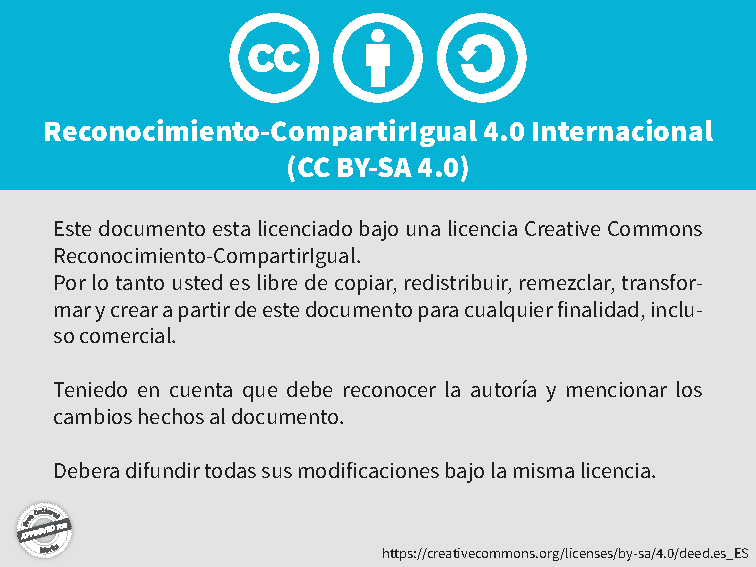
\includepdf[pages=1]{../Licencia_Diapositiva.pdf}}
\end{frame}
}


\begin{frame}[fragile]{Funciones Seno y Coseno}
\begin{center}
%	\begin{animateinline}[autoplay,loop,nomouse,poster=first]{24}
%		\multiframe{359}{nAngle=0+1}{
%			\begin{tikzpicture}
%			\draw[thick,-latex,blue] (-3,0) -- (3,0) node[right] {$x$};
%			\draw[thick,-latex,blue] (0,-3) -- (0,3) node[above] {$y$};
%			\draw[red,thick] (0,0) circle (2.5);
%			\draw[ultra thick,cyan] (0,0) -- (0,0 |- \nAngle:2.5) node[midway,left] {$\sin(\alpha)$};
%			\draw[ultra thick,orange] (0,0) -- (\nAngle:2.5 |- 0,0) node[midway,below] {$\cos(\alpha)$};
%			\draw[densely dotted,orange] (\nAngle:2.5) -- (\nAngle:2.5 |- 0,0);
%			\draw[densely dotted,cyan] (\nAngle:2.5) -- (0,0 |- \nAngle:2.5);
%			\draw[thick,green] (0.5,0) arc (0:\nAngle:0.5);
%			\draw[thick,green,opacity=0] (0.7,0) arc (0:\nAngle:0.7) node[midway,opacity=1] {$\alpha$};
%			\draw[ultra thick,red,-latex] (0,0) -- (\nAngle:2.5);
%			\end{tikzpicture}
%		}
%	\end{animateinline}
\end{center}
\end{frame}

\begin{frame}{¿Que es {\lmr\LaTeX}?}{}
{\lmr\LaTeX} es un sistema de composición de textos de calidad artística y tipográfica. Es usado muy habitualmente en el mundo científico debido a todas sus características y facilidad de trabajo.\pause\\[2em]

{\lmr\LaTeX} es un conjunto de macros de {\lmr\TeX}, publicado bajo la licencia {\it{\lmr L}PPL}, {\it{\lmr\LaTeX} Project Public License}. Por lo cual es {\em Software Libre} y gratuito.
\end{frame}

\section{Clases}
\begin{frame}{Clases del documento}{}
Al trabajar en un documento escrito con {\lmr\LaTeX} debemos tener en cuenta la clase del documento en el cual queremos trabajar, la clase más usada generalmente es \texttt{\textbf{article}}.\pause\\[2em]

Las clases «estándares» de {\lmr\LaTeX} son:
\begin{itemize}[<+->]
	\item {\color{Ired}\texttt{article}}: para artículos.
	\item {\color{Ired}\texttt{report}}: para reportes.
	\item {\color{Ired}\texttt{book}}: para libros.
	\item {\color{Ired}\texttt{letter}}: para las cartas.
	\item {\alt<+->{\color{black!30!Igreen}\textbf{\texttt{beamer}}}{\color{Ired} \texttt{slides}}}: para las presentaciones.
\end{itemize}
\end{frame}

\begin{frame}[fragile]{Clases del documento}{}
Para indicar la clase del documento a {\lmr\LaTeX} solo debemos de escribir en nuestro código:
\begin{center}
	\lstinline|\documentclass{<clase>}|
\end{center}
\pause
Donde \texttt{<clase>} es cualquiera de las clases ya mencionadas, u otras personalizadas o descargadas.
\end{frame}

\section{Estructura del código}
\begin{frame}[fragile]{Estructura del código}{}
La estructura básica del código de cualquier documento es muy sencilla, siempre es la misma.\pause

\begin{enumerate}[<+->]
	\item Primero se coloca el comando \lstinline|\documentclass{<clase>}| con la clase escogida.
	\item Desde aquí encontramos el \alert{\bf preámbulo} hasta que se encuentra la orden \lstinline|\begin{document}|.
	\item Después tenemos el \alert{\bf cuerpo del documento} hasta encontrar la orden \lstinline|\end{document}|, todo lo que se encuentra después de esto es ignorado por {\lmr\LaTeX}.
\end{enumerate}\pause[5]

Se debe tener cuidado al escribir, ya que existen comandos los cuales solo funcionan en una sección del código.
\end{frame}

\begin{frame}[fragile]{Estructura del código}{Código}
De manera más visual esto seria:
\begin{lstlisting}
\documentclass{<clase>}

Preámbulo ...

\begin{document}

Documento ...

\end{document}
\end{lstlisting}
\end{frame}

\section{Títulos}
\begin{frame}[fragile]{Títulos}{}
Al empezar a escribir, con cualquiera de las clases, necesitamos colocar el titulo de nuestro documento.\pause\\[2em]

Esto lo logramos mediante las ordenes:
\begin{itemize}
	\item \lstinline|\title{<título>}|
	\item \lstinline|\author{<autor o autores>}|
	\item \lstinline|\date{<fecha>}|
\end{itemize}\pause\vspace{2em}

Y para colocarlos en el documento de forma general, podemos hacerlo mediante la orden \lstinline|\maketitle|
\end{frame}

\begin{frame}[fragile]{Títulos}{}
Al escribir esto ya en un documento con la clase \alert{\bf articulo}, de manera normal, podemos obtener esto.\\[1em]

\begin{columns}
	\begin{column}{0.5\linewidth}
		{\small
\begin{lstlisting}
\documentclass{article}

\title{Título}
\author{John Doe}
\date{\today}

\begin{document}
  \maketitle
\end{document}
\end{lstlisting} }
	\end{column}
	\vline
	\hspace{1em}
	\begin{column}{0.5\linewidth}
		{\lmr\centering
		{\LARGE Título \par}
		\vspace{3em}
		{\large\vspace{.75em}
		\begin{tabular}[t]{c}
		John Doe
		\end{tabular}\par}
		\vskip 1.5em
		{\large \today \par}}
	\end{column}
\end{columns}
{\color{Ired} Código}\hfill{\color{Ired} Vista}
\end{frame}

\section{Capítulos-Partes, Secciones, etc.}
\begin{frame}{Capítulos-Partes, Secciones, etc.}{}
Al escribir cualquier tipo de documento siempre es bueno llevar una estructura e intentar no romperla a lo largo de este.\pause\\[2em]

En {\lmr\LaTeX} esto se logra mediante los comandos:
\begin{itemize}[<+->]
	\item \texttt{\textbackslash{}chapter\{<título>\}} para las clases \alert{\bf libro} y \alert{\bf reporte} \\
	\texttt{\textbackslash{}part\{<título>\}} para la clase \alert{\bf articulo}.
	\item \texttt{\textbackslash{}section\{<título>\}}
	\item \texttt{\textbackslash{}subsection\{<título>\}}
	\item Etc.
\end{itemize}
\end{frame}

\begin{frame}{Capítulos-Partes, Secciones, etc.}{}
Siempre que utilizamos estas ordenes {\lmr\LaTeX} las numera de forma automática, teniendo en cuenta que siguen un orden estructural.\pause

\begin{center}
	\begin{tikzpicture}
	\coordinate (zero) at (0,0);
	\node[red,above] (part) at (zero.north) {Parte};
	\node[red,below] (chapter) at (zero.south) {Capítulo};
	
	\node[blue] (sec) at (2,-1.5) {Sección};
	
	\node[cyan] (subsec) at (4,0) {Sub-Sección};
	
	\node[orange] (subsubsec) at (6,-1.5) {Sub-Sub-Sección};
	
	\draw[-latex,shorten <= 1cm,very thick] (zero) -- (sec);
	\draw[-latex,very thick] (sec) -- (subsec);
	\draw[-latex,very thick] (subsec) -- (subsubsec);
	\end{tikzpicture}
\end{center}\pause

Generalmente se suelen utilizar hasta las \alert{\bf sub-secciones}, pero es posible llegar, hasta los \alert{\bf sub-párrafos}.
\end{frame}

\section{El resumen}
\begin{frame}{El Resumen}{}
El resumen es una parte importante de cualquier trabajo escrito.\\[2em]

En {\lmr\LaTeX} existe el entorno \texttt{abstract} para las clases \texttt{article} y \texttt{report}. En este entorno podremos escribir el resumen de nuestro documento, con un margen más pequeño, y con el título que lo identifica.
\end{frame}

\begin{frame}[fragile]{El Resumen}
Al escribir esto en un documento con clase \alert{\bf articulo} obtenemos.\\[1em]

\begin{columns}
	\begin{column}{0.5\linewidth}
		{\small
\begin{lstlisting}
\documentclass{article}
\begin{document}
  \begin{abstract}
    Este es un pequeño
    resumen de este
    documento.
  \end{abstract}
  Texto normal de
  nuevo...
\end{document}
\end{lstlisting} }
	\end{column}
	\vline
	\hspace{1em}
	\begin{column}{0.5\linewidth}
		{\lmr{\small
		\begin{center}
			{\bfseries \abstractname\vspace{-.5em}}
		\end{center}
		\begin{quotation}
			\textup{Este es un pequeño
				resumen de este
				documento.}
		\end{quotation} }
		\hspace{2ex}Texto normal de nuevo... }
	\end{column}
\end{columns}
{\color{Ired} Código}\hfill{\color{Ired} Vista}
\end{frame}

\section{Familias, Estilos y Formas}
\begin{frame}{Familias, Estilos y Formas}{Familias}
{\lmr\LaTeX} ofrece una gran variedad de familias tipográficas donde se encuentran:\pause

\begin{itemize}[<+->]
	\item \alert{\bf\lmr Serif}, \alert{\bf\lmr Romana} o \alert{\bf\lmr Con Serifa}.\\
	\hspace*{2ex}Es la fuente por defecto de casi todo documento.
	\item \alert{\bf\lmss Sans Serif}, \alert{\bf\lmss Paloseco} o \alert{\bf\lmss Sin Serifa}.
	\item \alert{\lmtt Typewriter} o \alert{\lmtt mono-espaciada}.
\end{itemize}
\end{frame}

\begin{frame}[fragile]{Familias, Estilos y Formas}{Familias}
Para indicar a {\lmr\LaTeX} por cual de las familias debe cambiar, se pueden utilizar las ordenes siguientes:

\begin{center}
	\begin{tabular}{cc}
		\multirow{3}{*}{\lmr Serif} & \lstinline|\textrm{texto}| \\
		& \lstinline|{\rm texto}| \\
		& \lstinline|{\rmfamily texto}| \\ \hline
		%
		\multirow{3}{*}{\lmss Sans Serif} & \lstinline|\textsf{texto}| \\
		& \lstinline|{\sf texto}| \\
		& \lstinline|{\sffamily texto}| \\ \hline
		%
		\multirow{3}{*}{\lmtt Typewriter} & \lstinline|\texttt{texto}| \\
		& \lstinline|{\tt texto}| \\
		& \lstinline|{\ttfamily texto}|
	\end{tabular}
\end{center}
\end{frame}

\begin{frame}{Familias, Estilos y Formas}{Estilos y Formas}
{\lmr\LaTeX} tambien ofrece una gran variedad de formas y estilos tipográficos donde se encuentran:

\begin{itemize}[<+->]
	\item \alert{\lmr Upright} o \alert{\lmr Derecha}.
	\item \alert{\bf\lmr Bold} o \alert{\bf\lmr Negrita}.
	\item \alert{\it\lmr Italic} o \alert{\it\lmr Italica}.
	\item \alert{\sl\lmr Slanted} o \alert{\sl\lmr Inclinada}.
	\item \alert{\sc\lmr Small Caps} o \alert{\sc\lmr Versalitas}.
\end{itemize}
\end{frame}

\begin{frame}[fragile]{Familias, Estilos y Formas}{Estilos y Formas}
Para indicar a {\lmr\LaTeX} por cual de las familias debe cambiar, se pueden utilizar las ordenes siguientes:

\begin{center}
	\begin{tabular}{cc}
		\multirow{2}{*}{\lmr Upright} & \lstinline|\textup{texto}| \\
		& \lstinline|{\upshape texto}| \\ \hline
		%
		\multirow{3}{*}{\bf\lmr Bold} & \lstinline|\textrm{texto}| \\
		& \lstinline|{\bf texto}| \\
		& \lstinline|{\bfseries texto}| \\ \hline
		%
		\multirow{3}{*}{\it\lmr Italic} & \lstinline|\textit{texto}| \\
		& \lstinline|{\it texto}| \\
		& \lstinline|{\itshape texto}|
	\end{tabular}
\end{center}
\end{frame}

\begin{frame}[fragile]{Familias, Estilos y Formas}{Estilos y Formas}
Para indicar a {\lmr\LaTeX} por cual de los estilos o las formas debe cambiar, se pueden utilizar las ordenes siguientes:

\begin{center}
	\begin{tabular}{cc}
		\multirow{3}{*}{\sl\lmr Slanted} & \lstinline|\textsl{texto}| \\
		& \lstinline|{\sl texto}| \\
		& \lstinline|{\slshape texto}| \\ \hline
		%
		\multirow{3}{*}{\sc\lmr Small Caps} & \lstinline|\textsc{texto}| \\
		& \lstinline|{\sc texto}| \\
		& \lstinline|{\scshape texto}|
	\end{tabular}
\end{center}
\end{frame}

\begin{frame}[fragile]{Familias, Estilos y Formas}{Énfasis}
Se puede aclarar que las combinaciones de familias, estilos y formas son validas, y en la mayoría de los casos, conmutativas, pero no todas son posibles.\pause\\[2em]

Si necesitamos enfatizar una parte del texto, lo más apropiado es utilizar las ordenes \lstinline|{\em texto}| o \lstinline|\emph{texto}|, ya que estas dependen de cada familia, estilo o forma. Por lo que en cada caso escogerá la mejor opción.
\end{frame}

\section{Tamaño de fuente}
\begin{frame}[fragile]{Tamaño de la fuente}{}
En {\lmr\LaTeX} existen varias formas de cambiar el tamaño de la fuente.\pause\\[2em]
Los más básicos son los siguientes comandos:
\begin{center}
	\begin{tabular}{cc}
		\lstinline|\tiny| & {\tiny\lmr Muestra} \\
		\lstinline|\scriptsize| & {\scriptsize\lmr Muestra} \\
		\lstinline|\footnotesize| & {\footnotesize\lmr Muestra} \\
		\lstinline|\small| & {\small\lmr Muestra} \\
		\lstinline|\normalsize| & {\normalsize\lmr Muestra} \\
	\end{tabular}\vline
	\begin{tabular}{cc}
		\lstinline|\large| & {\large\lmr Muestra} \\
		\lstinline|\Large| & {\Large\lmr Muestra} \\
		\lstinline|\LARGE| & {\LARGE\lmr Muestra} \\
		\lstinline|\huge| & {\huge\lmr Muestra} \\
		\lstinline|\Huge| & {\Huge\lmr Muestra} \\
	\end{tabular}
\end{center}
\end{frame}

\begin{frame}[fragile]{Tamaño de la fuente}{}
Otra forma para cambiar el tamaño de la fuente del documento es mediante las opciones de \lstinline|\documentclass|.\\[2em]\pause

Estas opciones pueden ser \verb|10pt|, \verb|11pt| o \verb|12pt|, con el significado habitual de todo editor. Estas opciones son aplicadas de manera general al documento.
\end{frame}

\section{Paquetes {\tt fontenc} e {\tt inputenc}}
\begin{frame}[fragile]{Paquetes {\tt fontenc} e {\tt inputenc}}{}
Debido a algunas condiciones al momento de crear {\lmr\TeX} y {\lmr\LaTeX} no es posible insertar de manera regular los caracteres especiales como \alert{ñ} o \alert{á}.\pause\\[2em]

Para colocarlas se debe utilizar las ordenes \verb|\~n| para \alert{ñ} y \verb|\'a| para \alert{á}. Lo cual es muy lento al momento de escribir, y de utilizar algún programa de corrección ortográfica.
\end{frame}

\begin{frame}[fragile]{Paquetes {\tt fontenc} e {\tt inputenc}}{}
Para poder utilizar estos símbolos de manera natural en el documento, vamos a incluir los paquetes {\tt fontenc} e {\tt inputenc} en el preámbulo del documento.\pause\\[2em]

\begin{lstlisting}
\usepackage[T1]{fontenc}
\usepackage[utf8]{inputenc}
\end{lstlisting}\vspace{2em}

De esta forma podremos escribir la mayoría de caracteres especiales sin problemas y de manera nativa.
\end{frame}

\section{{\lmr\LaTeX} en español}
\begin{frame}[fragile]{{\lmr\LaTeX} en español}{}
Al escribir en un documento, colocar títulos y demás rótulos, estos tienen el formato e idioma ingles.\pause\\[1em]

Para cambiarlo, y utilizar rótulos en español es necesario incluir el paquete \verb|babel|.\pause\\[1em]

\begin{lstlisting}
\usepackage[spanish]{babel}
\end{lstlisting}\pause\vspace{1em}

Para cambiar el rotulo de \alert{Cuadro} por \alert{Tabla} debemos colocar la opción \verb|es-tabla|. Y para seguir lo dicho por la RAE ASALE en Ortografía de la Lengua Española (2010), utilizaremos la opción \verb|es-nodecimaldot|.
\end{frame}

\section{Separación del texto}
\begin{frame}[fragile]{Separación del texto}{}
Para generar estructura en cualquier texto es necesario dividirlo en párrafos.\pause\\[1em]

En {\lmr\LaTeX} existen varias formas de generar párrafos.\pause\\[1em]

Los más básicos y útiles son:
\begin{itemize}[<+->]
	\item \lstinline|\par|
	\item \lstinline|\\|
	\item \lstinline|\newline|
	\item \lstinline|\linebreak|
\end{itemize}\pause[7]\vspace{1em}

Aunque existen muchos más comandos que realizan esta tarea, como dejar una línea en blanco entre dos textos.
\end{frame}

\begin{frame}[fragile]{Separación del texto}{}
Cada uno de los comandos anteriores funciona de manera diferente. Por ejemplo, el comando \lstinline|\linebreak| estira proporcionalmente los espacios entre las palabras hasta tocar el margen derecho.\pause\\[2em]

\begin{center}
	\fbox{
		\begin{minipage}{0.7\linewidth}\lmr
			% Se puede obtener el mismo resultado con
			% Esta línea será estirada.\linebreak
			% pero enviara un mensaje de advertencia.
			Esta\hfill{}línea\hfill{}será\hfill{}estirada.\\
			Mientras esta no.
		\end{minipage} }\\[1ex]

\begin{lstlisting}
Esta línea será estirada.\linebreak
Mientras esta no.
\end{lstlisting}
\end{center}
\end{frame}

\section{Opciones del documento}
\begin{frame}[fragile]{Opciones del documento}{}
Podemos modificar muchas cosas de nuestro documento mediante las opciones de la orden \lstinline|\documentclass[]{}|.\pause\\[1em]

Lo más general suele ser:
\begin{itemize}[<+->]
	\item El \alert{\bf Tamaño de la fuente}.
	\item El \alert{\bf tamaño del papel}.
	\item La \alert{\bf orientación del papel}.
	\item El \alert{\bf número de columnas}.
	\item La \alert{\bf forma del título}.
	\item Impresión a \alert{\bf una} o \alert{\bf dos} caras.
	\item El \alert{\bf tipo de impresión}.
	\item Ubicación de la \alert{\bf página de título}.
\end{itemize}
\end{frame}

\begin{frame}{Opciones del documento}{Tamaño de la fuente}
Originalmente solo podemos escoger entre 3 tamaños para nuestro documento.\pause\\[2em]

\begin{center}
	{\setlength{\tabcolsep}{5mm}
	\begin{tabular}{ccc}
		{\tt 10pt} & {\tt 11pt} & {\tt 12pt} \\
		{\fontsize{10}{12}\lmr Muestra} & {\fontsize{11}{13.2}\lmr Muestra} & {\fontsize{12}{14.4}\lmr Muestra}
	\end{tabular} }
\end{center}\pause\vspace{1em}

Aunque es posible que alguna clase o paquete que utilices te habiliten nuevos tamaños.
\end{frame}

\begin{frame}{Opciones del documento}{Tamaño del papel}
Al escoger el tamaño del papel, solo tendremos 6 tipos.\pause\\[2em]

\begin{center}
	\begin{tabular}{c|cc}
		\hline
		Orden & Ancho & Alto \\
		\hline
		{\tt letterpaper} & 8.5 pulgadas & 11 pulgadas \\
		{\tt legalpaper} & 8.5 pulgadas & 14 pulgadas \\
		{\tt executivepaper} & 7.25 pulgadas & 10.5 pulgadas \\
		{\tt a4paper} & 21 centímetros & 30 centímetros \\
		{\tt a5paper} & 15 centímetros & 21 centímetros \\
		{\tt b5paper} & 18 centímetros & 25 centímetros \\
		\hline
	\end{tabular}
\end{center}
\end{frame}

\begin{frame}{Opciones del documento}{Orientación del papel}
Las orientaciones del papel son muy sencillas, solo existen 2.\pause\\[2em]

\begin{itemize}[<+->]
	\item {\tt portrait}: que refiere a \emph{retrato}, en \alert{\bf vertical}.
	\item {\tt landscape}: que refiere a \emph{paisaje}, en \alert{\bf horizontal}.
\end{itemize}
\end{frame}

\begin{frame}{Opciones del documento}{Número de columnas}
En el número de columnas, de manera normal, solamente hay 2 opciones.\pause\\[2em]

\begin{itemize}[<+->]
	\item {\tt onecolumn}: para una columna.
	\item {\tt twocolumn}: para dos columnas iguales.
\end{itemize}\pause[4]\vspace{2em}

Puedes también incluir el paquete {\tt multicol}, el cual te permite tener más control sobre las columnas.
\end{frame}

\begin{frame}{Opciones del Documento}{Página de título}
También puedes escoger si prefieres o no una página separada para el título.\pause\\[2em]

\begin{itemize}[<+->]
	\item {\tt titlepage}: con lo cual el título se dispondrá en una página separada.
	\item {\tt notitlepage}: con lo cual el título se dispondrá junto al texto.
\end{itemize}
\end{frame}

\begin{frame}{Opciones del documento}{Impresión a una o dos caras}
Podremos cambiar los margenes \emph{izquierdo} y \emph{derecho} de las páginas \emph{pares} e \emph{impares}.\pause\\[2em]

\begin{itemize}[<+->]
	\item {\tt oneside}: con lo cual los margenes son iguales tanto para páginas pares como impares.
	\item {\tt twoside}: con lo cual se reflejan los margenes en páginas pares e impares.
\end{itemize}
\end{frame}

\begin{frame}{Opciones del documento}{Tipo de impresión}
Al hablar del tipo de impresión nos referimos a la versión del documento que estamos compilando.\pause\\[2em]

\begin{itemize}[<+->]
	\item {\tt draft}: que seria un borrador del documento, la compilación es rápida, pero el documento no se ve completo.
	\item {\tt final}: es la versión final del documento. Donde se muestran todos los elementos del documento.
\end{itemize}
\end{frame}

\begin{frame}{Opciones del documento}{Primera página de cada capítulo}
Cuando se escribe una Parte, o un capítulo se puede elegir en que lado del documento aparezca.\pause\\[2em]

\begin{itemize}[<+->]
	\item {\tt openright}: los títulos de partes y capítulos aparecen siempre del lado derecho del documento.
	\item {\tt openany}: los títulos de partes y capítulos pueden aparecer a cualquier lado del documento.
\end{itemize}
\end{frame}

\begin{frame}{Bibliografía}
\nocite{*}
\bibliographystyle{babplain}
\bibliography{biblio}
\end{frame}
\end{document}
